\chapter{Data}
\clearpage

\section{Types of Data}
	
	\begin{itemize}
		\item {\bf Data set: } collection of data objects.
		\item {\bf Data Objets: } often called record, point, vector, pattern, event, case,
		sample, observation or entity. Data objects are described by a number of attributes
		that capture the basic characteristics of an object.
		\item {\bf Attributes: } other names used are variable, characteristic, field, feature, 
		or dimension. An attribute is a property or characteristic of an object that may
		vary, either from one object to another or from time to another.
		\item {\bf Measurement scale: } is a rule (function) that associates a numerical or
		symbolic value with an attribute of an object. It is important to understand the 
		mesurement. An attribute can be an integer like ID and age. They are both integers, 
		but it does not mean that we can calculate the average ID numer like we can calculate
		the average age. Note that is common to refer to the type of an attribute as the
		{\bf type of a measurement scale}.
	\end{itemize}

	\subsection*{Types of Attributes}
	{\bf Categorical types (Qualitative):} Nominal and Ordinal

	{\bf Numeric types (Quantitative):} Interval and Ratio

		\begin{figure}[H]
			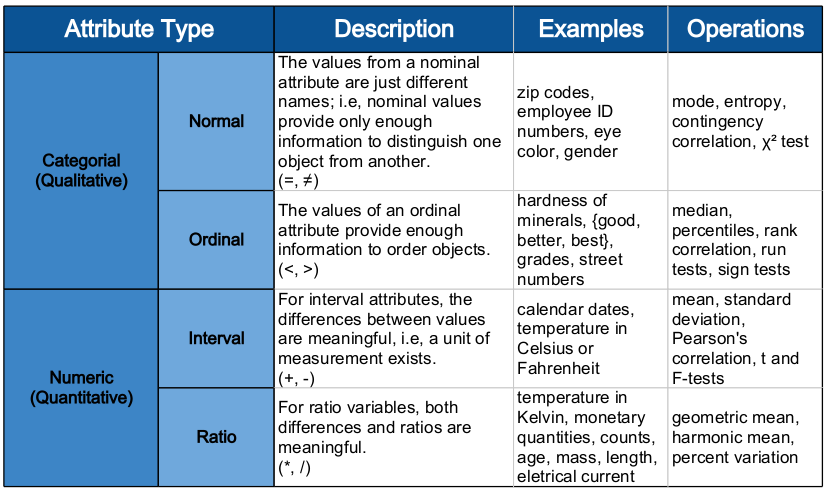
\includegraphics[width=\textwidth]{pics/typeOfAttributes.png}
		\end{figure}

	\clearpage
	\subsection*{Transformations}

		The types of attributes can be described in terms of transformations that
		do not change the meaning of an attribute. 

		\begin{figure}[H]
			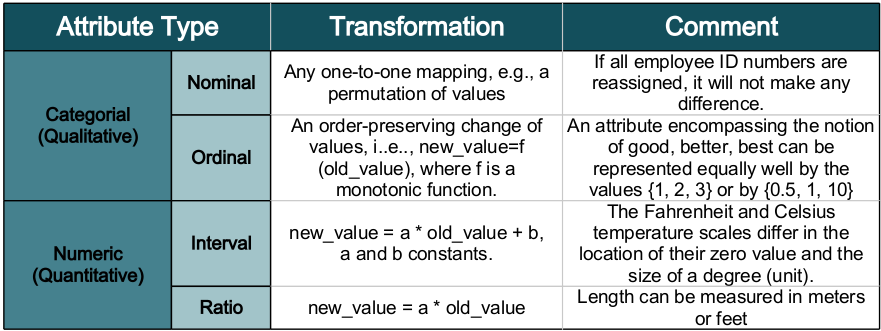
\includegraphics[width=\textwidth]{pics/transformations.png}
		\end{figure}

	\subsection*{Attributes by the Number of Values}

	An independent way of distinguishing between attributes is by the number of values
	they can take.

	\begin{itemize}
		\item {\bf Discrete:} A discrete attribute has a finite or countably infinite
		set of values. {\bf Binary attributes} are a special case of discrete attributes. 
		\item {\bf Continnuous:} A continuous attribute is one whose values are real numbers.
		\item {\bf Asymmetric:} For asymmetric attributes, only presence - a non-zero attribute
		value - is regarded as important. Binary attributes where only non-zero values are 
		important are called asymmetric binary attibutes. We can take a look at a list of all 
		courses at NTNU. If we look at a particular student, the chance for a particular student
		have taken a exam in a course from the whole list is quite small. It is only the non-zero
		values that are important. 
	\end{itemize}

	\clearpage
	\section{Type of Data Sets}

		\subsection*{General Characteristics of Data Sets}
			\begin{itemize}
				\item {\bf Dimensionality:}
				\item {\bf Sparsity:}
				\item {\bf Resolution:}
			\end{itemize}

		\subsection*{Record Data}
			\begin{itemize}
				\item {\bf Transactions or Market Basket Data:}
				\item {\bf The Data Matrix:}
				\item {\bf The Sparse Data Matrix:}
			\end{itemize}

		\subsection*{Graph-Based Data}
			\begin{itemize}
				\item {\bf Data with Relationships among Objects:}
				\item {\bf Data with Objects Thar Are Graphs:}
			\end{itemize}

		\subsection*{Ordered Data}
			\begin{itemize}
				\item {\bf Sequential Data (temporal data):}
				\item {\bf Sequence Data:}
				\item {\bf Time Series Data:}
				\item {\bf Spatial Data:}
			\end{itemize}

		\subsection*{Handling Non-Record Data}